\subsection{Salidas de diez pasos}

\begin{figure}[htbp]
\centering
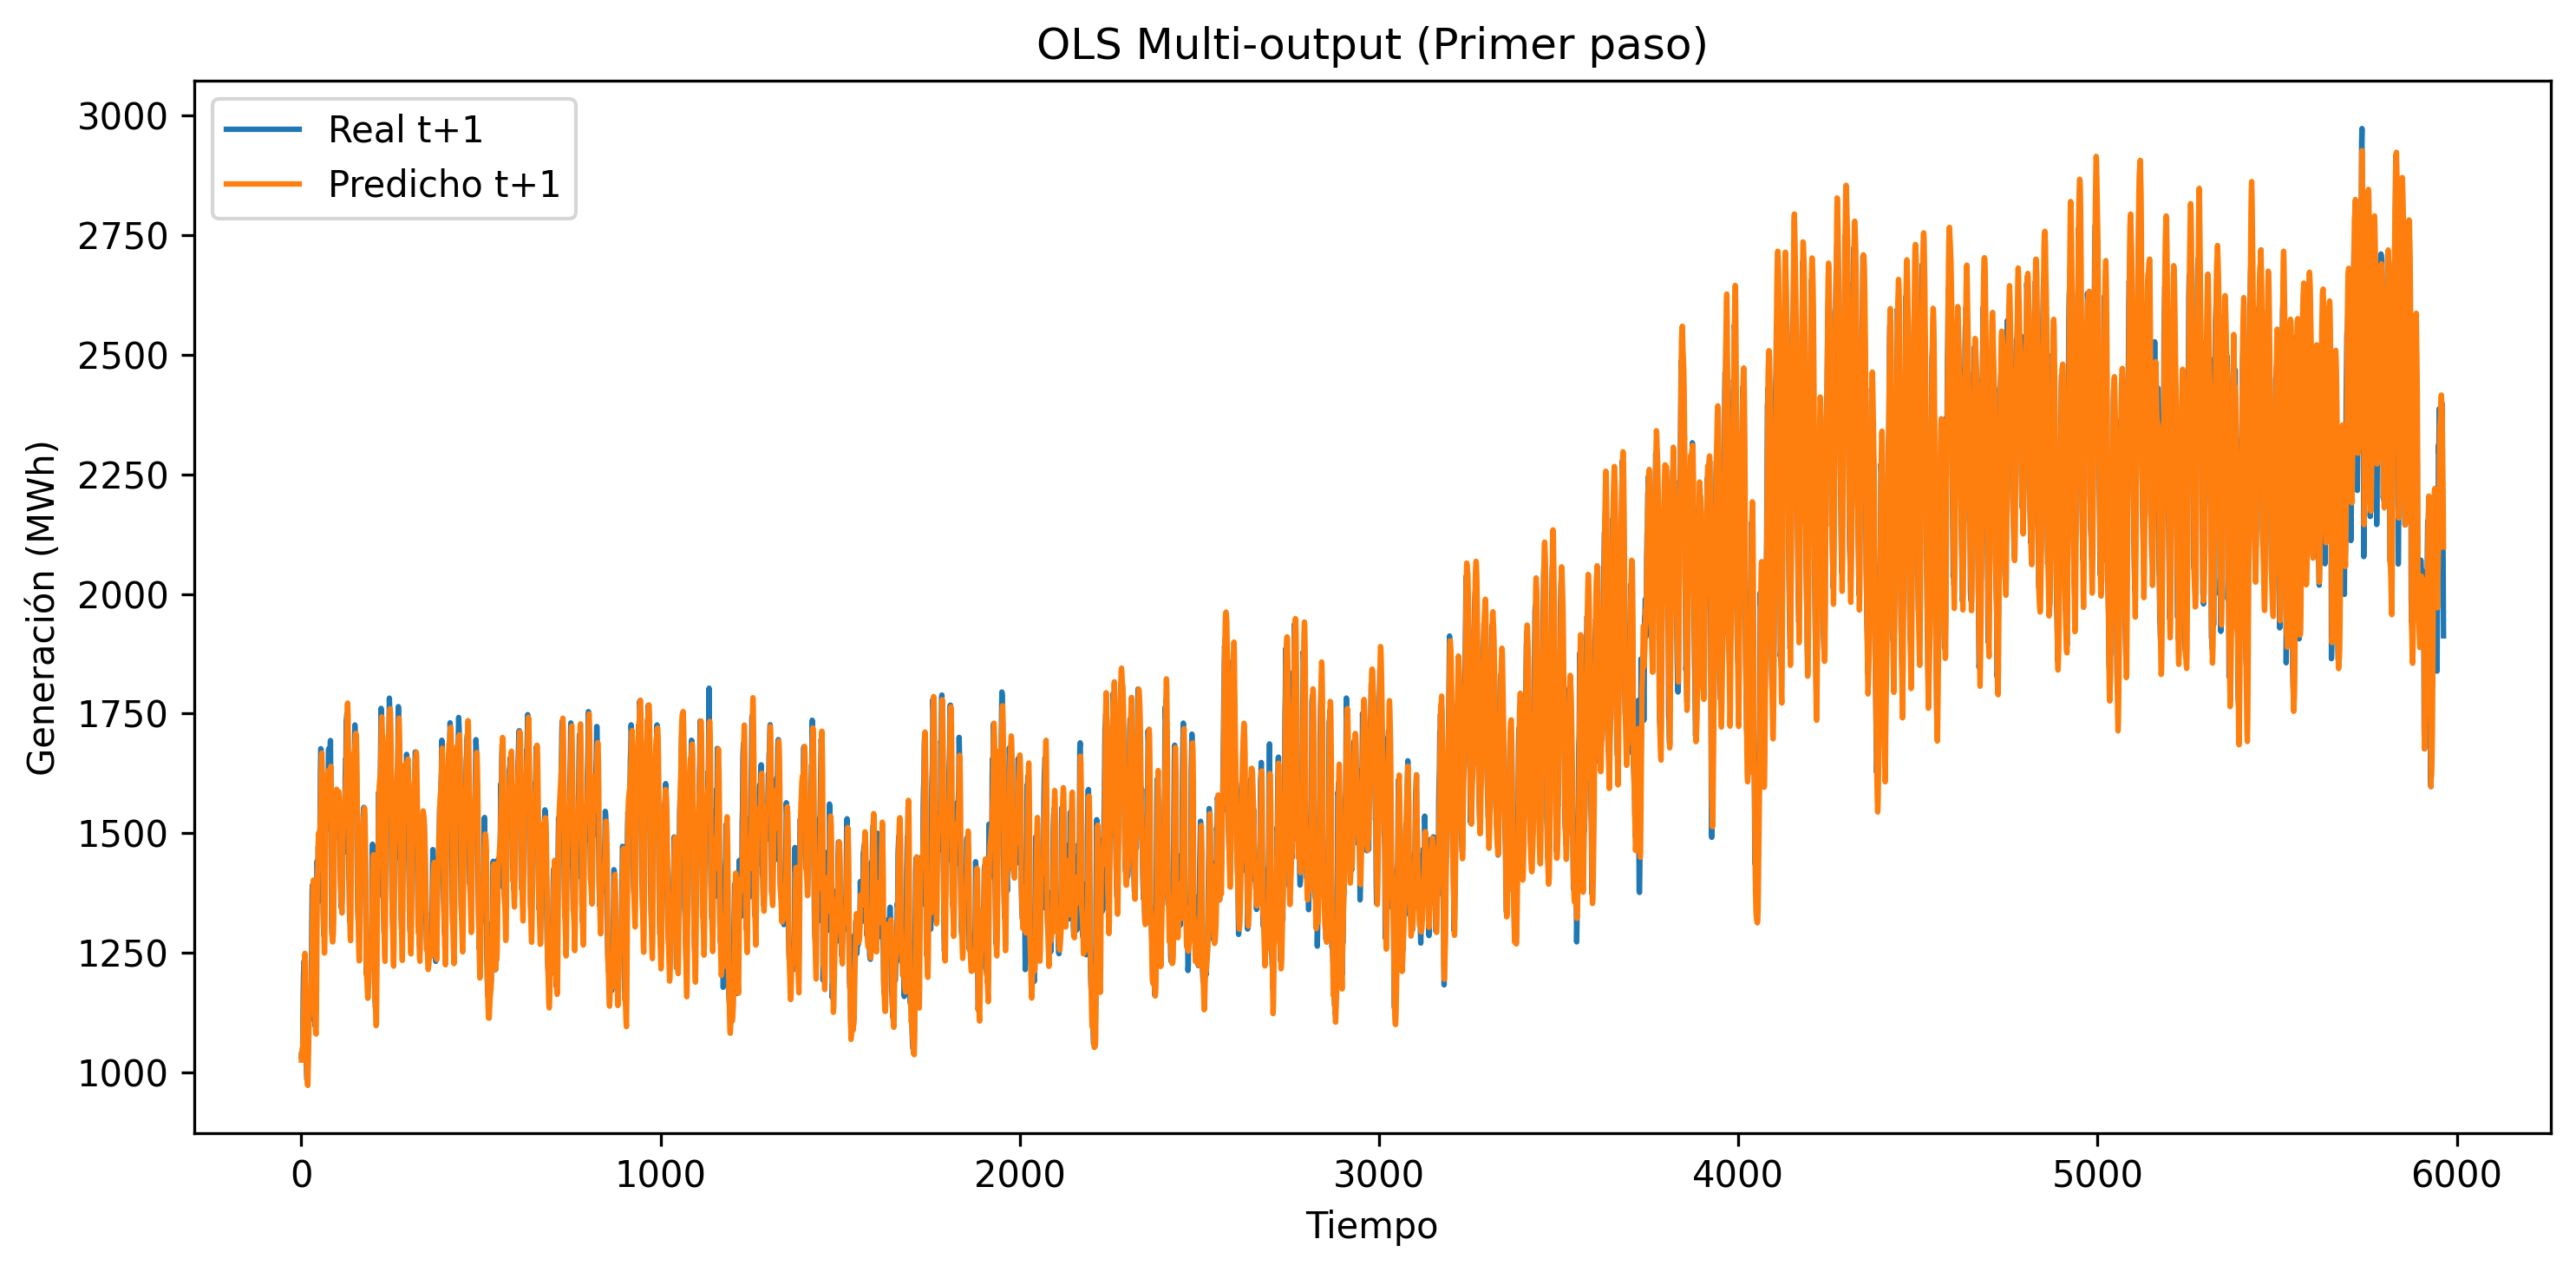
\includegraphics[width=\textwidth]{figuras/05_resultados/ols_diez_pasos.png}
\caption{Primer componente de la salida múltiple de OLS. La construcción de las respuestas incluye datos del intervalo evaluado.}
\label{fig:ols-multi}
\end{figure}

\begin{figure}[htbp]
\centering
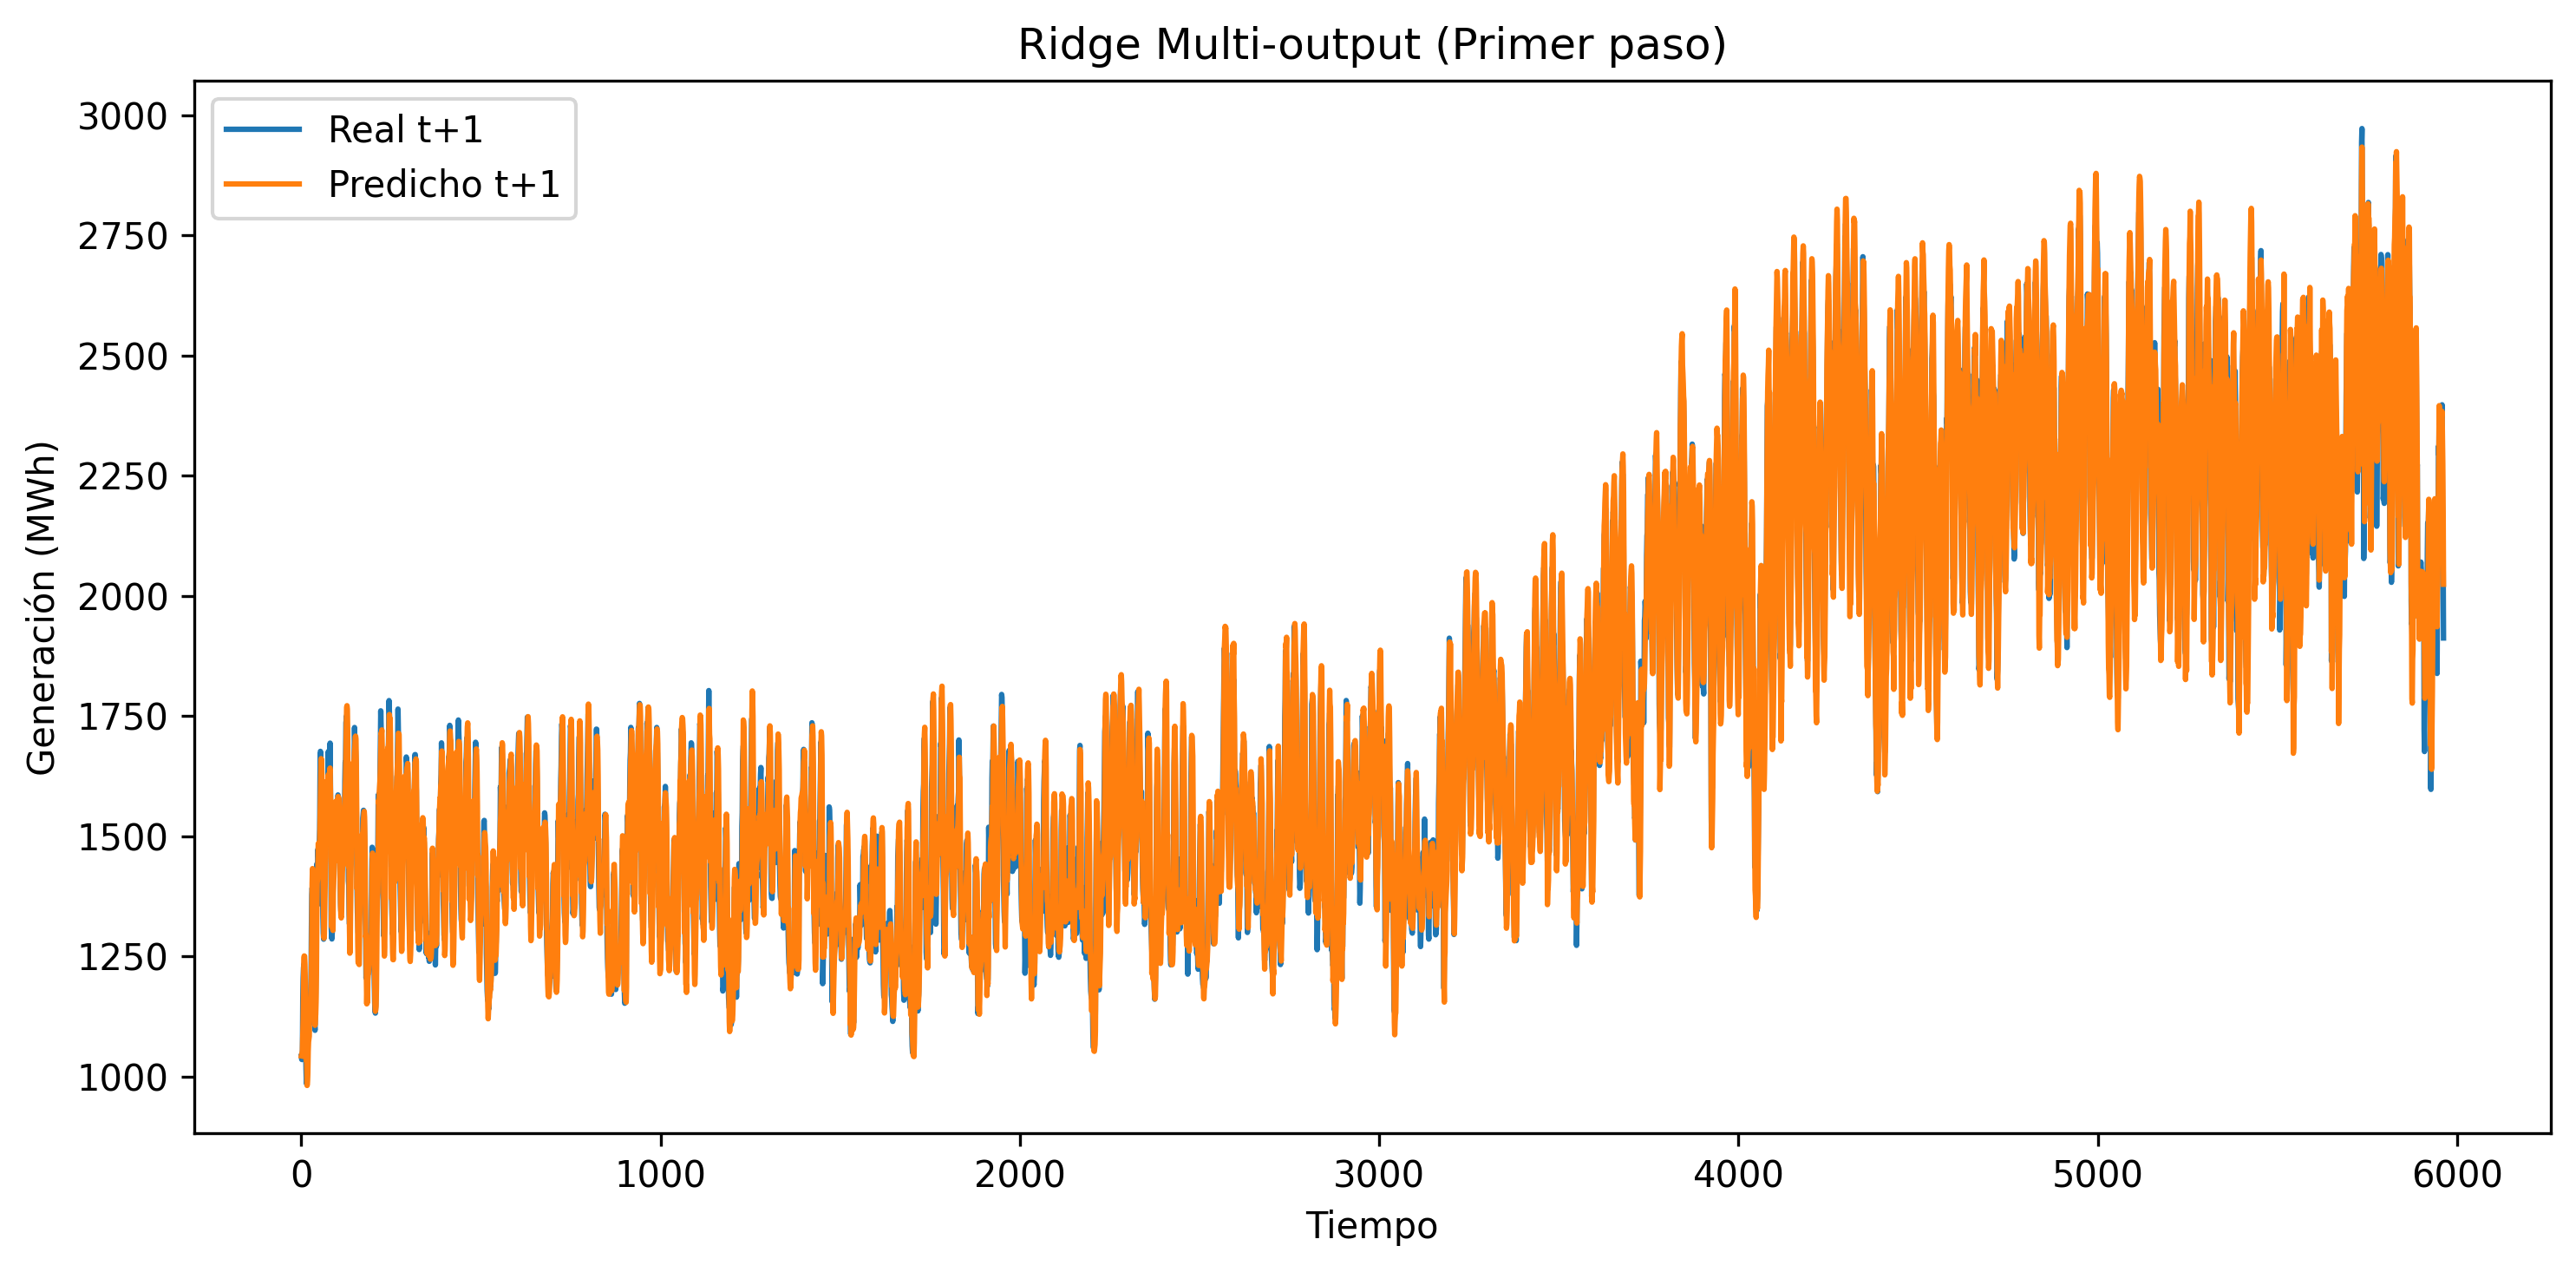
\includegraphics[width=\textwidth]{figuras/05_resultados/ridge_diez_pasos.png}
\caption{Primer componente de la salida múltiple de Ridge. Esta gráfica no representa el desempeño de los diez horizontes por separado.}
\label{fig:ridge-multi}
\end{figure}

Las figuras~\ref{fig:ols-multi} y~\ref{fig:ridge-multi} muestran cercanía entre las curvas del primer componente. Sin embargo, la fuga de información identificada en la subsección~\ref{subsec:lineales-multi} condiciona su interpretación: la coincidencia no demuestra capacidad de generalización a datos futuros. Tampoco permite inferir el comportamiento de los pasos segundo a décimo, ausentes en las imágenes.
